\documentclass[tikz,border=5pt]{standalone}
\usepackage[T1]{fontenc}
\usepackage[utf8]{inputenc}
\usepackage{lmodern}
\usepackage{amsmath,amssymb}
\usepackage{siunitx}
\usepackage{xcolor}
\usepackage{tikz}
\usetikzlibrary{
  arrows.meta,
  backgrounds,
  calc,
  decorations.pathreplacing,
  fit,
  matrix,
  positioning,
  shapes.geometric
}

\sisetup{
  detect-all = true,
  group-minimum-digits = 4,
}

\definecolor{TdcBlue}{HTML}{5B739F}
\definecolor{TdcRed}{HTML}{A35E66}
\definecolor{TdcLilac}{HTML}{8D83A7}
\definecolor{TdcCyan}{HTML}{82A9B8}
\definecolor{TdcGray}{HTML}{6D7175}
\definecolor{TdcBlack}{HTML}{202124}

\colorlet{TdcBlueFill}{TdcBlue!7}
\colorlet{TdcRedFill}{TdcRed!7}
\colorlet{TdcLilacFill}{TdcLilac!8}
\colorlet{TdcCyanFill}{TdcCyan!10}
\colorlet{TdcGrayFill}{black!3}
\colorlet{TdcGuide}{black!32}
\colorlet{TdcGuideLight}{black!18}

\tikzset{
  >=Latex,
  every picture/.style = {line join=round, line cap=round},
  every node/.style = {font=\small, text=TdcBlack},
  module/.style = {
    draw=black!72,
    fill=white,
    line width=0.50pt,
    rounded corners=0.8pt,
    minimum height=9mm,
    minimum width=22mm,
    align=center,
    inner sep=3pt
  },
  module gray/.style = {module, fill=TdcGrayFill},
  module slow/.style = {module, draw=TdcBlue, fill=TdcBlueFill},
  module fast/.style = {module, draw=TdcRed, fill=TdcRedFill},
  module ctrl/.style = {module, draw=TdcLilac, fill=TdcLilacFill},
  module io/.style = {module, draw=TdcCyan, fill=TdcCyanFill},
  domain box/.style = {
    draw=black!32,
    fill=black!1.5,
    line width=0.40pt,
    rounded corners=1.0pt,
    inner sep=4pt
  },
  domain label/.style = {
    font=\scriptsize\itshape,
    text=black!70
  },
  signal/.style = {-{Latex[length=2.2mm,width=1.5mm]}, draw=black!72, line width=0.60pt},
  signal slow/.style = {signal, draw=TdcBlue},
  signal fast/.style = {signal, draw=TdcRed},
  signal ctrl/.style = {signal, draw=TdcLilac},
  signal io/.style = {signal, draw=TdcCyan!80!black},
  signal dashed/.style = {signal, dashed},
  bidir/.style = {<->, draw=black!72, line width=0.55pt},
  guide/.style = {draw=TdcGuide, line width=0.35pt},
  guide dashed/.style = {guide, dashed},
  fine mark/.style = {draw=black!60, line width=0.40pt},
  brace note/.style = {
    decorate,
    decoration={brace, amplitude=3.0pt},
    draw=black!55,
    line width=0.40pt
  },
  note/.style = {
    font=\scriptsize,
    inner sep=1.5pt,
    fill=white,
    text=black!78
  },
  axis label/.style = {
    font=\scriptsize,
    text=black!72
  },
  lane label/.style = {
    font=\small,
    text=black!82
  },
  legend box/.style = {
    draw=black!60,
    line width=0.40pt,
    minimum width=4mm,
    minimum height=3mm
  },
  timeline block/.style = {
    draw=black!72,
    line width=0.45pt,
    minimum height=7.5mm,
    rounded corners=0.5pt,
    align=center,
    inner sep=2pt
  },
  timeline capture/.style = {timeline block, draw=TdcRed, fill=TdcRedFill},
  timeline snapshot/.style = {timeline block, draw=TdcLilac, fill=TdcLilacFill},
  timeline drain/.style = {timeline block, draw=TdcCyan!80!black, fill=TdcCyanFill},
  timeline free/.style = {timeline block, draw=black!60, fill=TdcGrayFill},
}

\newcommand{\DomainLabel}[2]{%
  \node[domain label, anchor=north west] at ($(#1.north west)+(0.10,-0.10)$) {#2};
}

\newcommand{\LegendItem}[4]{%
  \begin{scope}[shift={#1}]
    \node[legend box, fill=#2, anchor=west] at (0,0) {};
    \node[axis label, anchor=west] at (0.18,0) {#4};
  \end{scope}
}


\begin{document}
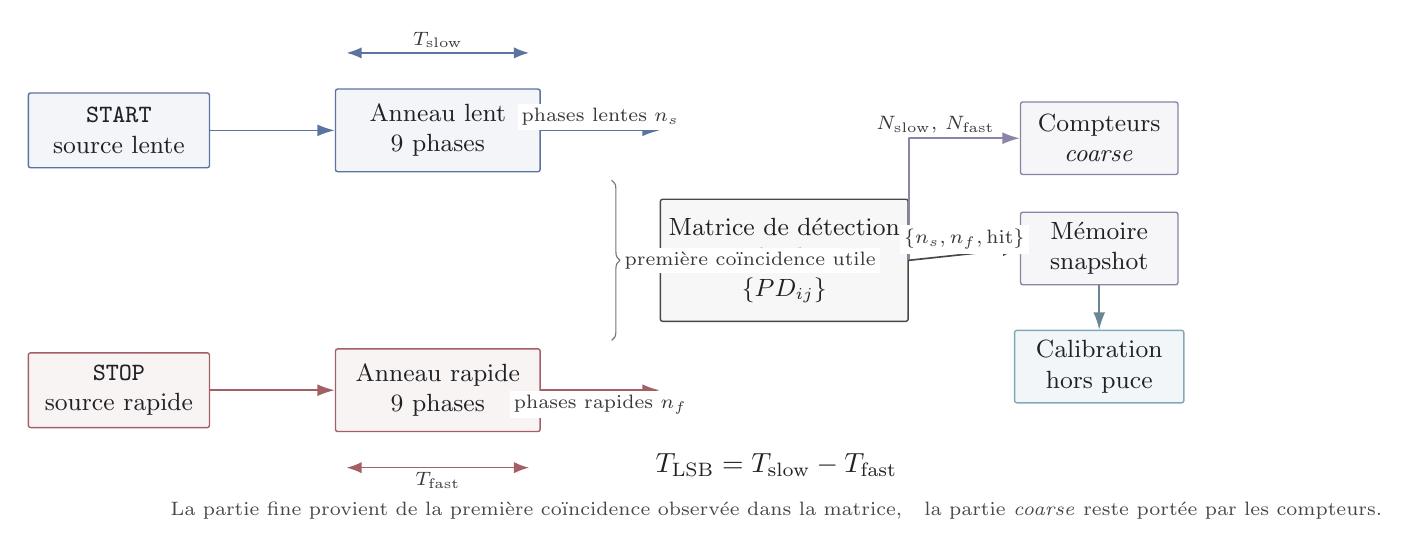
\begin{tikzpicture}[x=1cm,y=1cm]
  \node[module slow, minimum width=2.30cm, minimum height=0.95cm] (start) at (0.0,1.65) {\texttt{START}\\source lente};
  \node[module fast, minimum width=2.30cm, minimum height=0.95cm] (stop) at (0.0,-1.65) {\texttt{STOP}\\source rapide};

  \node[module slow, minimum width=2.60cm, minimum height=1.05cm] (slowring) at (4.05,1.65) {Anneau lent\\$9$ phases};
  \node[module fast, minimum width=2.60cm, minimum height=1.05cm] (fastring) at (4.05,-1.65) {Anneau rapide\\$9$ phases};

  \node[module gray, minimum width=2.75cm, minimum height=1.55cm] (matrix) at (8.45,0.0) {Matrice de détection\\multiphase\\$\{PD_{ij}\}$};

  \node[module ctrl, minimum width=2.00cm, minimum height=0.92cm] (counters) at (12.45,1.55) {Compteurs\\\textit{coarse}};
  \node[module ctrl, minimum width=2.00cm, minimum height=0.92cm] (snapshot) at (12.45,0.15) {Mémoire\\snapshot};
  \node[module io, minimum width=2.15cm, minimum height=0.92cm] (calib) at (12.45,-1.35) {Calibration\\hors puce};

  \draw[signal slow] (start.east) -- (slowring.west);
  \draw[signal fast] (stop.east) -- (fastring.west);
  \draw[signal slow] (slowring.east) -- node[note, above] {phases lentes $n_s$} (matrix.west|-slowring.east);
  \draw[signal fast] (fastring.east) -- node[note, below] {phases rapides $n_f$} (matrix.west|-fastring.east);

  \draw[signal ctrl] (matrix.east) |- node[note, pos=0.62, above] {$N_{\mathrm{slow}},\,N_{\mathrm{fast}}$} (counters.west);
  \draw[signal] (matrix.east) -- node[note, above] {$\{n_s,n_f,\mathrm{hit}\}$} (snapshot.west);
  \draw[signal io] (snapshot.south) -- (calib.north);

  \draw[bidir, draw=TdcBlue] ($(slowring.north west)+(0.15,0.45)$) -- node[note, above] {$T_{\mathrm{slow}}$} ($(slowring.north east)+(-0.15,0.45)$);
  \draw[bidir, draw=TdcRed] ($(fastring.south west)+(0.15,-0.45)$) -- node[note, below] {$T_{\mathrm{fast}}$} ($(fastring.south east)+(-0.15,-0.45)$);

  \draw[brace note] ($(slowring.south east)+(0.90,-0.10)$) -- node[note, right=3pt] {première coïncidence utile} ($(fastring.north east)+(0.90,0.10)$);

  \node[font=\normalsize] at (8.35,-2.60) {$T_{\mathrm{LSB}} = T_{\mathrm{slow}} - T_{\mathrm{fast}}$};
  \node[axis label, align=center] at (8.35,-3.18)
    {La partie fine provient de la première coïncidence observée dans la matrice,\quad
     la partie \textit{coarse} reste portée par les compteurs.};
\end{tikzpicture}
\end{document}
